Esamineremo ora alcuni modelli che sono stati costruiti per finalizzare la descrizione del nucleo.

Una classificazione di alcuni modelli nucleari in base al tipo di interazione tra nucleoni è la seguente:
\begin{multicols}{2}
	\begin{center}
		Models with strong interaction between nucleons:
	\end{center}
	\begin{itemize}
		\item \textbf{Liquid drop model} (Modello a goccia);
		\item \textbf{Shell model} (Modello a shell);
		\item $ \alpha-$particle model.
	\end{itemize}
   \begin{center}
	   Nucleons interact with the nearest neighbors and practically don‘t move: mean free path \[ \lambda \ll R\]
   \end{center}
	\columnbreak

	\begin{center}
		Models of non-interacting nucleons :
	\end{center}
	\begin{itemize}
		\item \textbf{Fermi gas model} (Modello a gas di fermioni);
		\item Optical model (Modello ottico).
	\end{itemize}
	\begin{center}
		Nucleons move freely inside the nucleus: mean free path \[ \lambda \sim R\]
	\end{center}
\end{multicols}
\begin{center}
($ R$ being the nuclear radius)
\end{center}
\section{Il modello nucleare a goccia}\label{sec:il-modello-nucleare-a-goccia}
Il grafico (Fig.~\ref{fig:en-legame-graph}) della energia di legame media per nucleone commentato in precedenza
contiene un certo numero di importanti indicazioni
sulle proprietà della forza nucleare che sono alla base di un primo
modello del nucleo - suggerito da Bohr nel 1935 - fondato essenzialmente
sul \textbf{raggio finito} della interazione nucleare.
Similmente alle forze intramolecolari a corto raggio nei liquidi,
tale fatto determina una certa analogia tra il comportamento dei nucleoni
nel nucleo e le diverse porzioni di un fluido meccanico incomprimibile, ragione che
giustifica il nome spesso usato di \textbf{modello a goccia}.
\begin{figure}
	\centering
	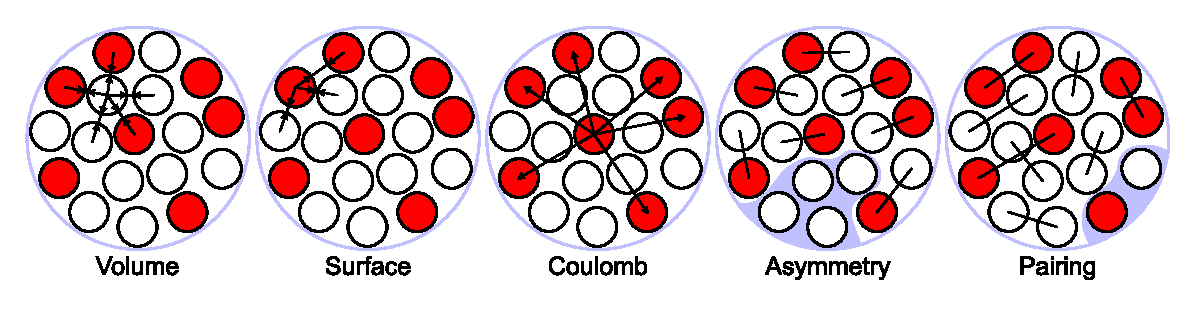
\includegraphics{figs/liquid-drop-model}
	\caption{Rappresentazione grafica del significato fisico dei termini presenti nel nuclear liquid drop model.}
	\label{fig:liquid-drop-model}
\end{figure}

Il suddetto modello ha base \textbf{fenomenologica}; la sola ipotesi
dell'andamento a corto raggio della forza non è sufficiente a
giustificare l'andamento reale

Come accennato, l'energia di legame tende ad assumere rapidamente il
valore medio di circa \(8MeV\) per nucleone (saturazione) il che indica
una energia di legame del nucleo proporzionale al numero di nucleoni
\begin{equation}
	\frac{B}{A} \simeq 8 MeV \qquad B \simeq 8 MeV \times A
    \label{eq:saturation-binding-energy-per-nucleon}
\end{equation}
Ora, se la forza nucleare si comportasse come una forza a lungo
raggio (come le forze gravitazionali o elettromagnetiche) ogni nucleone
interagirebbe con tutti i rimanenti altri per cui dovremmo attenderci
una energia di legame del nucleo tendenzialmente \emph{proporzionale al numero
di coppie} di nucleoni e dunque quadratica in A
\[
	B \propto \frac{A(A-1)}{2} \propto A^{2} \qquad
\]
Poiché i dati sulla energia di legame escludono questo tipo di
comportamento, dobbiamo concludere che ogni nucleone del nucleo
interagisce solo con un numero di fisso di nucleoni vicini per cui
concludiamo che \textbf{l'interazione forte ha un raggio d'azione finito}
dell'ordine di grandezza delle dimensioni del nucleone stesso.

Tale conclusione è in perfetto accordo con i dati sulla sezione d'urto
di neutroni su nuclei analizzati in precedenza che indicavano un \textbf{volume
nucleare proporzionale al numero di nucleoni}, ovvero una densità
volumetrica di nucleoni uniforme sul volume nucleare, fatto spiegabile
solo postulando la esistenza di una forza d'interazione tra nucleoni a
corto raggio.

Il primo tentativo di superare questo limite consiste nell'introdurre un
termine, sulla base della (\ref{eq:saturation-binding-energy-per-nucleon})
\begin{equation}
	B = a_{v} A
   \label{eq:volume-term-drop-model}
\end{equation}
dove la costante \(a_{v}\) viene detta \textbf{termine di volume}.
\begin{marginfigure}
	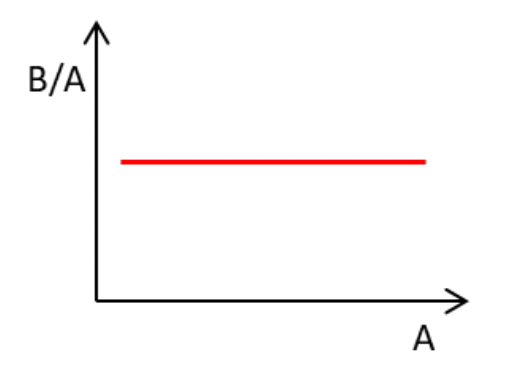
\includegraphics{figs/goccia1}
	%    \caption{This is a margin figure.}
	\label{fig:goccia1}
\end{marginfigure}
Con un tale andamento \(B / A\) , però, si finisce per ottenere una sovrastima
del volume.
La deviazione più rilevante si manifesta per valori piccoli di A dove
l'energia media di legame è molto inferiore a quanto previsto dalla
formula.
\bigskip

Si può allora osservare che, assumendo la forza nucleare a
corto raggio, si deve tenere conto che un nucleone prossimo alla
superficie del nucleo interagirà con un numero di nucleoni inferiore a
quello con cui interagirebbe qualora si trovasse all'interno del nucleo
stesso.
Ciò comporta che i nucleoni superficiali contribuiranno in
misura minore alla energia di legame nucleare di quelli interni al
volume.
Assumendo il nucleo di \textbf{forma sferica}, il numero di
nucleoni prossimi alla superficie sarà proporzionale a \(R^{2}\).
Dalla trattazione precedente (\ref{eq:nuclear-radius-skin}) sappiamo che (omettendo il termine di `skin'
nucleare) \begin{gather*}
	R_{\text{nuc}} = r_{0}A^{1/3}\\
	4 \pi R^{2} = 4 \pi (r_{0}A^{1/3})^2 \implies R_{\text{nuc}} \propto A^{2/3}
\end{gather*} per cui vi deve essere un termine che deve provocare un difetto di
energia di legame proporzionale ad \(A^{2/3}\): \[
	B = a_{v}A - a_{s}A^{2/3}
\] dove la costante \(a_{s}\) viene detta \textbf{termine di
	superficie}.
L'andamento di \(B / A\) con questa ulteriore correzione
può apprezzarsi a lato.
\begin{marginfigure}
	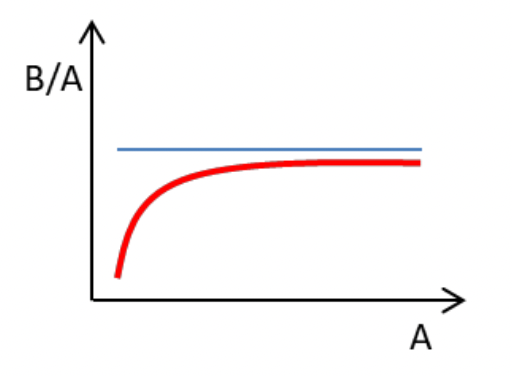
\includegraphics{figs/goccia2}
	%    \caption{This is a margin figure.}
	\label{fig:goccia2}
\end{marginfigure}
\bigskip

Un ulteriore miglioramento può essere ottenuto tenendo presente che i
protoni del nucleo si \emph{respingono elettrostaticamente} diminuendo
quindi il lavoro necessario per separarli dal nucleo stesso.
In effetti
se, per assurdo, si avesse un nucleo composto solo di protoni(senza
neutroni) il lavoro da spendere per mantenerne la configurazione sarebbe
sicuramente maggiore.

Ipotizzando una \emph{distribuzione di protoni uniforme} nel volume
nucleare (ricordiamo essere sferico dall'ipotesi precedente), otteniamo
la seguente espressione del lavoro fatto dalle forze coulombiane
repulsive per separare la carica nucleare
\begin{gather*}
	\delta L = \int _{R}^{\infty} \left( \frac{q \delta q}{4 \pi \epsilon_{0}r^{2}}  \hat{\bm{r}} \right)(dr \hat{\bm{r}})=
	- \frac{q \delta q}{4 \pi \epsilon_{0}r} \bigg |_{R}^{\infty} =
	- \frac{q \delta q}{4 \pi \epsilon_{0}R}\\
	q = \rho \frac{ 4}{3} \pi R^{3} \qquad \delta q = \rho 4 \pi R^{2} dR\\
	\delta L = \frac{1}{4 \pi \epsilon_{0}R}\left( \rho \frac{ 4}{3}\pi R^{3} \right)(\rho 4 \pi R^{2} dR) = \frac{4 \pi \rho^{2}}{3 \epsilon_{0}}R^{4}dR\\
	L = \int \delta l = \frac{4 \pi \rho^{2}}{15 \epsilon_{0}}R_{0}^{5} \qquad Q = \rho \frac{ 4}{3} \pi R_{0}^{3} = Ze\\
	L = \frac{3}{20 \pi \epsilon_{0}} \frac{Q^{2}}{R_{0}} = \frac{3e^{2}}{20 \pi \epsilon_{0}r_{0}} \frac{Z^{2}}{A^{1/3}}
	\implies L \propto \frac{ Z^{2}}{A^{1/3}}
\end{gather*} Ne consegue che la energia di legame nucleare dovrà essere corretta
sottraendo un termine proporzionale a \(Z^{2} / A^{1/3}\) per cui
l'espressione dell'energia di legame acquisirà la forma seguente
\begin{equation}
	B = a_{v}A - a_{s}A^{2/3} - a_{c} \frac{Z^{2}}{A^{1/3}}
	\label{eq:coulomb-term-drop-model}
\end{equation}
 dove la nuova costante \(a_{c}\) viene detta \textbf{termine
	coulombiano}.
Il termine coulombiano deve chiaramente annullarsi per
\(A=1\)(non c'e interazione elettrostatica) per cui l'unica forma
possibile è
\begin{equation}
	L \propto \frac{Z(Z-1)}{A^{1/3}} \quad
   \label{eq:work-to-seperate-uniformly-distributed-protons}
\end{equation}
\begin{marginfigure}
	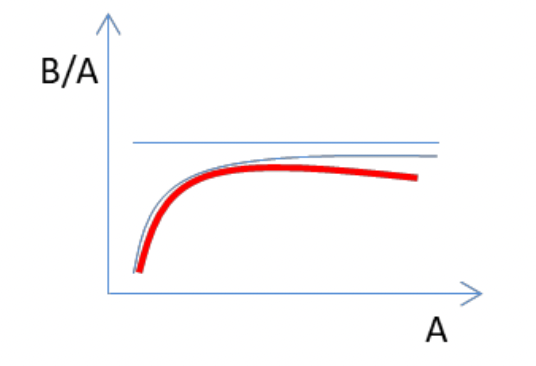
\includegraphics{figs/goccia3}
	%    \caption{This is a margin figure.}
	\label{fig:goccia3}
\end{marginfigure}

L'andamento $B / A$ risulta ulteriormente migliorato (si tenga presente
che nei nuclei stabili si ha approssimativamente \(Z=A/2\) per cui il
termine coulombiano sottrae un contributo crescente con \(A^{5/3}\)).

Se il modellino fenomenologico costruito finora fosse completo dovremmo
concludere che i nuclei più stabili(\(B= B_{max}\)) sono quelli con
\(Z=0\) ovvero i nuclei di soli neutroni.
Tale fatto è palesemente
contraddetto dai dati sperimentali i quali mostrano che i nuclei stabili
hanno un numero di protoni di poco inferiore a quello dei neutroni (la
differenza tra neutroni e protoni tende a crescere con il numero
atomico).
Il nostro modello -- basato sulla natura a corto raggio della
interazione nucleare -- non offre alcun appiglio per dare un fondamento
fisico a questo stato di cose che potrà essere spiegato solo nel
contesto della meccanica quantistica attraverso il \emph{principio di
	esclusione di Pauli}.
In questa situazione l'unica possibilità è quella
di introdurre un termine `ad hoc' capace di descrivere i dati
sperimentali.

Bisogna quindi fare in modo che il modello ci dica che i nuclei piu
stabili sono quelli con lo stesso numero di protoni e neutroni.
Raggiungiamo l'obiettivo introducendo un nuovo termine del tipo:
\[
	Z \simeq \frac{A}{2} \quad A - 2Z \simeq 0
\]
Ricordando però che con il crescere di \(A, Z\) tende ad essere via
via più piccolo di \(A/2\) (il quoziente protoni/neutroni diminuisce con
\(A\)), tale termine correttivo dovrà seguire una legge inversa ad A
modulata da un qualche esponente.
I dati indicano che la prima potenza è
sufficiente per cui abbiamo la seguente espressione della energia di
legame nucleare
\[
	B = a_{v}A - a_{s}A^{2/3} - a_{c} \frac{Z(Z-1)}{A^{1/3}} - \frac{a_{a}(A-2Z)^{2}}{A}
\]
dove la nuova costante \(a_{a}\) viene detta \textbf{termine di asimmetria}.
Notiamo che la presenza di \(A\) a denominatore è
giustificata osservando l'andamento dei dati sperimentali nel grafico
visto in precedenza:tanto piu \(A\) è grande tanto piu \(B / A\) devia
dalla tangente alla curva (quindi verso il basso).

Per completare il modello è necessario tenere conto di un ulteriore
proprietà dei nuclei.
I dati sperimentali mostrano che tra i 254 nuclei
stabili noti ben 148 sono del tipo \textbf{pari-pari} (un numero pari
sia di protoni che di neutroni), 101 sono del tipo \textbf{pari-dispari}
(un numero pari di protoni ma dispari di neutroni o viceversa) e solo 5
sono del tipo dispari-dispari (riportati in tabella \ref{tab:odd-odd-stable-nuclei}).
\begin{table}
	\centering
	\begin{tabular}{|c|}
		\hline
		$\isotope[2][1]{\mathlarger{H}}$ \\ \hline
		$\isotope[6][3]{\mathlarger{Li}}$ \\ \hline
		$\isotope[10][5]{\mathlarger{B}}$ \\ \hline
		$\isotope[14][7]{\mathlarger{N}}$ \\ \hline
		$\isotope[180m][73]{\mathlarger{Ta}}$ \\ \hline
	\end{tabular}
	\caption{Tabella dei nuclei stabili con both $ A,Z$ dispari. L'$m$ ad apice indica la metastabilità del nuclide. \\
	Si veda \url{https://en.wikipedia.org/wiki/Metastability#Nuclear_physics} a tale proposito.}
	\label{tab:odd-odd-stable-nuclei}
\end{table}

Similmente, tra i 35 nuclei a lunga vita media si hanno 22 pari-pari, 9 pari-dispari e 4
dispari-dispari.

Tali dati sembrano suggerire che per qualche motivo la forza forte tra
nucleoni da luogo a nuclei di maggiore stabilità quando vengono legati
\textbf{numeri pari} di neutroni e protoni, un fatto che trova una sua
diretta evidenza nell'andamento della energia di legame per nucleone
della serie isotopica dello xenon in Figura~\ref{fig:binding-energy-xenon}.
Tali dati sembrano suggerire che per qualche motivo la forza forte tra nucleoni da luogo a nuclei di maggiore stabilità
quando vengono legati \textbf{numeri pari} di neutroni e protoni, un fatto che trova una sua diretta evidenza nell’andamento della energia di legame per nucleone della serie isotopica dello xenon.
\begin{marginfigure}
	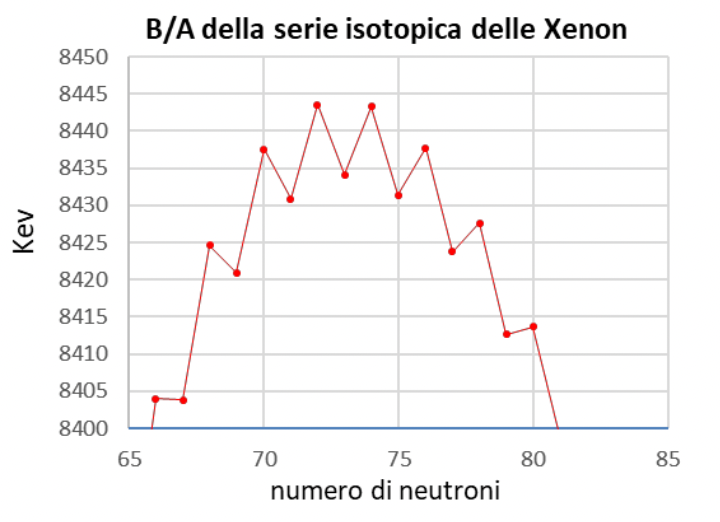
\includegraphics[scale = 1.5]{figs/goccia5}
	\caption{Andamento dell'energia di legame per la serie isotopica dello Xenon.}
	\label{fig:binding-energy-xenon}
\end{marginfigure}
Tenendo presente che il nucleo di Xenon ha \(Z=54\) protoni, si può
infatti constatare che gli isotopi con un numero pari di neutroni hanno
una maggiore energia di legame per nucleone.
Per rendere conto di questo
fatto si introduce un nuovo coefficiente detto di \textbf{pairing} \[
	a_{p} \frac{\delta}{A^{3/4}}
\] con \[
	\delta =
	\begin{cases}
		+1    \qquad  \text{pari-pari}       \\
		\ 0  \qquad  \ \ \text{pari-dispari} \\
		-1  \qquad  \text{dispari-dispari}
	\end{cases}
\] Giungiamo così alla seguente espressione complessiva della energia di
legame nucleare detta anche \textbf{formula semiempirica della energia
	di legame nucleare} o \textbf{formula di Weizsacker} della energia di
legame nucleare
\begin{equation}
	\boxed{    B = a_{v}A - a_{s}A^{2/3} - a_{c} \frac{Z(Z-1)}{A^{1/3}} - a_{a}\frac{(A-2Z)^{2}}{A} +     a_{p} \frac{\delta}{A^{3/4}}}
	\label{eq:weizsacker-formula}
\end{equation} Essa dipende da 5 parametri(vedi Fig.~\ref{fig:liquid-drop-model}) il cui valore numerico
viene determinato adattando la formula ai dati sperimentali di \(B/A\).

A titolo di esempio, una possibile combinazione di valori è la seguente(i
valori sono in \(MeV\)):
\[
	a_{v} = 15.5 \quad a_{s} = 16.8 \quad a_{c} = 0.72 \quad a_{a} = 23.0 \quad a_{p} = 34.0
\]
La formula della energia di legame nucleare è utile - come strumento di
calcolo - perchè suggerisce una prima interpretazione del nucleo e delle
forze che lo tengono insieme.

Da essa deduciamo che le forze tra nucleoni devono essere \textbf{molto
	intense} ma a \textbf{short range} (proprietà di saturazione), producono
una distribuzione spaziale tendenzialmente uniforme di nucleoni e
conducono ad una espressione della energia di legame con termini di
volume e superficie in analogia con quanto accade per i liquidi, ragione
che giustifica il nome spesso usato di \textbf{modello nucleare a
	goccia}.

Il \emph{modello a gas di fermioni} (giustificabile con considerazioni
quantomeccaniche) riesce a rendere conto del termine \(a_{a}\) mentre
fallisce per quello di pairing.
Vedremo, infine, che il \emph{modello a shell} sarà quello piu preciso.

%%%%%%%%%%%%%%%%%%%%%%%%%%%%%%%%%%%%%%%%%%%%%%%%%%%%%%%%%%%%%%%%%%%%%%%%%%%%%%%%%%%%%%%%%%%%%%%%%%%%%%%%%%%%%%%%%%%%%%%%
%%%%%%%%%%%%%%%%%%%%%%%%%%%%%%%%%%%%%%%%%%%%%%%%%%%%%%%%%%%%%%%%%%%%%%%%%%%%%%%%%%%%%%%%%%%%%%%%%%%%%%%%%%%%%%%%%%%%%%%%
%%%%%%%%%%%%%%%%%%%%%%%%%%%%%%%%%%%%%%%%%%%%%%%%%%%%%%%%%%%%%%%%%%%%%%%%%%%%%%%%%%%%%%%%%%%%%%%%%%%%%%%%%%%%%%%%%%%%%%%%
\section{Il nucleo come gas di fermioni}\label{sec:il-nucleo-come-gas-di-fermioni}



Il modello a goccia del nucleo - essenzialmente fondato sulla natura a corto raggio delle interazioni forti - riesce a descrivere alcune proprietà del nucleo tra le quali l’esistenza di una energia di legame con termini di volume, superficie e coulombiano.
Non riesce invece a rendere conto in nessun modo dei termini di asimmetria e accoppiamento, chiaramente richiesti dai dati sperimentali, ma che devono essere introdotti ‘a mano’ nella formula di Weizsacker.
Tale fatto dimostra che oltre alla natura a corto raggio delle interazioni forti, nel nucleo giocano un ruolo di rilievo altre proprietà trascurate dal modello a goccia, presumibilmente legate alla natura quantomeccanica dei suoi costituenti.
Il modello nucleare a gas di fermioni introduce nel gioco alcuni essenziali proprietà quantomeccaniche in una forma il più possibile semplificata.

\subsection{Aspetti generali}\label{sec:aspetti-generali}

Le considerazioni fisiche che conducono alla formulazione del modello a gas di fermioni possono essere riassunte nei seguenti punti:
\begin{itemize}
	\item l’interazione forte che lega protoni e neutroni nel nucleo è a corto raggio
	e dell’ordine del raggio dei nucleoni stessi;
	\item ogni nucleone sarà quindi soggetto alla forza forte dei nucleoni
	immediatamente a contatto che tenderanno così a disporsi con densità
	volumetrica approssimativamente costante;
	\item ciò comporta che la risultante delle forze agenti sul singolo nucleone sia
	mediamente nulla quando questo si trova all’interno al nucleo e mediamente non nulla e diretta verso il centro quando questo si trova sulla superficie del nucleo;
	\item riassumersi in una forza dipendente dalla posizione, nulla all’interno di un volume sferico di raggio $R$ (raggio nucleare) e non nulla e centrale sulla sua superficie;
	\item essendo $ \bm{F} = - grad \, U$, tale forza può essere descritta da un potenziale
	nullo all’interno del volume sferico di raggio R, che sale con una certa ripidità in corrispondenza della superficie sferica,
	fino a raggiungere un valore costante al di fuori di essa. \\
	In sintesi, una \textbf{buca sferica di potenziale di raggio R} all’interno della quale vanno a collocarsi sia i neutroni che i protoni.
\end{itemize}
\bisgkip

Dato questo assetto delle forze, la meccanica quantistica fa il resto.
Infatti sappiamo che
\begin{itemize}
	\item una particella microscopica vincolata a rimanere in una regione di spazio
	limitata (nel nostro caso all’interno della buca di potenziale) deve annullare la propria funzione d’onda più o meno sulla superficie di tale regione ed all’esterno di essa;
	\item ciò comporta la quantizzazione delle lunghezze d’onda di De Broglie dei neutroni e dei protoni e, con esse, della loro energia (fenomeno analogo alla quantizzazione delle lunghezze d’onda in una corda vibrante) cosicchè gli stati quantomeccanici vanno a costituire una serie discreta e numerabile;
	\item dato che protoni e neutroni hanno spin $s=\frac{1}{2}$, essi vanno a costituire due insiemi di fermioni identici soggetti alle restrizioni del principio di esclusione;
	\item organizzando la serie discreta degli stati quantomeccanici possibili secondo i valori crescenti delle loro energie, il principio di esclusione permette di collocare in ciascuno di essi un solo protone ed un solo neutrone;
	\item nello stato fondamentale di minima energia del nucleo, neutroni e protoni nucleari riempiranno allora dal basso tutti gli stati quantomeccanici fino ad un livello energetico massimo detto \textbf{livello di Fermi} (nello stato fondamentale di minima energia dunque, i neutroni ed i protoni non sono immobili ma possiedono una certa energia cinetica crescente).
\end{itemize}

Le precedenti considerazioni ci conducono a concludere che la \emph{natura della forza media nucleare}, combinata con la
\emph{natura quantomeccanica dei suoi costituenti}, \textbf{assimila il nucleo nel suo stato fondamentale ad un doppio
gas di neutroni e protoni in condizioni di massima degenerazione}.
Parliamo di `gas’ poiché neutroni e protoni – come si è detto – si muovono essenzialmente liberi all’interno del volume nucleare subendo le sole forze di contenimento delle pareti nucleari.
Il termine ‘doppio’ ricorda che le restrizioni del principio di esclusione si applicano separatamente ai protoni ed ai neutroni.
Infine, il termine ‘degenerazione’ si riferisce al fatto che gli stati quantomeccanici quantizzati si riempiono tutti a partire da quelli meno energetici fino al livello di Fermi.
Come noto, tale condizione si realizza nei \textbf{gas di fermioni identici alle bassissime temperature che trovano così una loro sorprendente relazione con il nucleo nel suo stato fondamentale}.
Da questo punto di vista la differenza è solo quantitativa poiché i gas quantomeccanici contano un numero di elementi dell’ordine del numero di Avogadro mentre il doppio gas nucleare risulta costituito da decine di unità un fatto che – come già osservato – rende sostanzialmente inapplicabili i metodi della meccanica statistica.

Nel prosieguo, l’approccio del modello a gas di fermioni verrà utilizzato per costruire una formula della energia di legame più evoluta di quella fornita dal modello a goccia nella speranza che la meccanica quantistica possa rendere conto dei termini introdotti in modo puramente fenomenologico nella formula di Weizsacker.

\subsection{La funzione d'onda dei nucleoni}\label{sec:funzione-onda-nucleoni}

Il primo passo è quello di scrivere la funzione d’onda di $N$ neutroni e $Z$ protoni soggetti alla buca di potenziale sferica che descrive la forza media agente su di loro all’interno del nucleo.
Senza perdere in generalità, possiamo semplificare i calcoli immaginando una \emph{buca di potenziale cubica di lato L} all’interno della quale si trova un emph{nucleone} (protone o neutrone) in uno stato quantomeccanico descritto da un’onda piana di De Broglie
\[
\psi(\bm{r},t) = A e^{ i(\bm{k} \cdot \bm{r} - \omega t) } =
Ae^{ \frac{i}{\hslash} (\bm{p} \cdot \bm{r} -Et)  } =
(Ae^{ \frac{i}{\hslash}p_{x}x }e^{ \frac{i}{\hslash}p_{y}y }e^{ \frac{i}{\hslash}p_{z}z })e^{ - \frac{i}{\hslash}Et }
\]
Con tutta evidenza, per descrivere correttamente lo stato quantomeccanico del nucleone, tale emph{funzione d’onda dovrà annullarsi sulla superficie cubica}.
Gli esponenziali complessi non possono annullarsi per cui è necessario ipotizzare che la funzione d’onda contenga solo le parti sinusoidali o cosinusoidali di tali esponenziali
\begin{equation}
	\psi(\bm{r},t) = A \sin\left(  \frac{1}{\hslash}p_{x}x \right) \sin\left(  \frac{1}{\hslash}p_{y}y \right) \sin\left(  \frac{1}{\hslash}p_{z}z \right) e^{ - \frac{i}{\hslash}Et }
	\label{eq:wave-function-nucleon-fermion-gas-non-normalized}
\end{equation}
In questa forma è agevole imporre l’annullamento della funzione d’onda sulle pareti della cavità nucleare ovvero sui piani $x=0$, $x=L$;  $y=0$, $y=L$; $z=0$, $z=L$.
Ragionando ad esempio lungo la direzione $x$ abbiamo le condizioni
\[
\frac{1}{\hslash} p_{x}x \big|_{x = 0,L} = 0
\]
sempre soddisfatta in $x=0$ e soddisfatta in $x=L$ solo se
\[
\frac{1}{\hslash}p_{x}L = n_{x} \pi \qquad n_{x} = 1,2, \dots, N
\]
Dato che condizioni analoghe si trovano immediatamente anche nelle direzioni y e z, giungiamo alla conclusione che le componenti cartesiane della \emph{quantità di moto} del nucleone soddisfano le seguenti \emph{condizioni di quantizzazione}
\begin{equation}
	p_{x} = n_{x} \frac{\pi \hslash}{L} \quad
	p_{y} = n_{y} \frac{\pi \hslash}{L} \quad
	p_{z} = n_{z} \frac{\pi \hslash}{L} \qquad
	n_{x},n_{y},n_{z} = 1,2, \dots , n
	\label{eq:quantized-momentum-fermions-gas}
\end{equation}
Come anticipato, ciò comporta che pure \emph{l’energia} del nucleone soddisfi la seguente \emph{condizione di quantizzazione}
\begin{equation}
	E = \frac{p^{2}}{2 M} = \frac{1}{2 M} \left( \frac{\pi \hslash}{L} \right)^{2} (n_{x}^{2} + n_{y}^{2}+n_{z}^{2}) \qquad
	n_{x},n_{y},n_{z} = 1,2, \dots , n
	\label{eq:energy-nucleon-fermions-gas}
\end{equation}
dove l'energia considerata è la cinetica in quanto nel modello che stiamo costruendo $ V(r) = 0$ per $ r< R$.
Sostituendo le (\ref{eq:quantized-momentum-fermions-gas}) nella (\ref{eq:wave-function-nucleon-fermion-gas-non-normalized})
ed imponendo la condizione di normalizzazione sul volume nucleare
\begin{gather*}
    \iiint_{V} |\psi(\bm{r},t) |^{2} \, dV = 1 \iff
1 = A^{2} \prod_{i = 1}^{3} \int_{0}^{L} \sin ^{2}\left( n_{x_{i}} \frac{\pi x_{i}}{L} \right) \, dx_{i}\\
    1 = A^{2} \left( \frac{L}{2} \right)^{3} \Longrightarrow A = \sqrt{ \frac{8}{L^{3}} }
\end{gather*}
otteniamo la \textbf{funzione d’onda del nucleone nel volume nucleare cubico di lato L}
\begin{equation}
	\psi(\bm{r},t) = \sqrt{ \frac{8}{L^{3}}} \sin\left( n_{x} \frac{\pi x}{L} \right) \sin\left( n_{y} \frac{\pi y}{L} \right)
	\sin\left( n_{z} \frac{\pi z}{L} \right) e^{ -\frac{i}{\hslash}Et }
	\label{eq:wave-function-nucleon-fermion-gas-normalized}
\end{equation}
Si comprende allora che gli stati quantomeccanici del nucleone vanno a costituire una \emph{sequenza discreta e numerabile di stati univocamente identificati da una terna ordinata di numeri naturali (non nulli e positivi)} $n_x, n_y, n_z$  \emph{detti numeri quantici dello stato}.

\subsection{Nucleoni e principio di esclusione} \label{sec:nucleoni-principio-di-esclusione}

Trovata l’espressione degli stati quantomeccanici di un generico nucleone nella cavità nucleare, vogliamo ora calcolare \emph{il numero di stati che possiedono una energia minore o uguale ad un certo prefissato valore}.
Con tutta evidenza - dato il legame esistente tra energia e quantità di moto – ciò equivale a calcolare il numero di stati che possiedono un modulo della quantità di moto minore od uguale ad un certo prefissato valore.

Premesso che il calcolo si base sulla stessa tecnica applicata a suo tempo al caso della radiazione elettromagnetica di cavità, si comincia \emph{introducendo uno spazio tridimensionale i cui punti rappresentano i vettori della quantità di moto che avranno così proiezioni} $p_x, p_y \ \text{e} \ p_z$.

Tenendo conto delle relazioni di quantizzazione della quantità di moto (\ref{eq:quantized-momentum-fermions-gas}), si comprende immediatamente che – in tale spazio – i valori delle quantità di moto accessibili al nucleone si collocano nel primo ottante sulle intersezioni di un grigliato tridimensionale di passo $\frac{\pi \hslash}{L}$.
A ciascuna di tali intersezioni corrisponde anche una determinata terna ordinata di numeri quantici $n_{x}, n_{y}$ e $n_{z}$ e, con essa, un determinato stato quantomeccanico.

Ciò premesso, si capisce che \textit{il numero di stati quantomeccanici aventi modulo della quantità di moto uguale o inferiore ad un prefissato valore}
$\tilde{p}$ è approssimativamente uguale al quoziente tra il volume dell’ottante di sfera di raggio $\tilde{p}$ ed il volumetto cubico del grigliato
\[
n_{s} = \frac{1}{8} \frac{ \frac{4}{3} \pi \tilde{p}^{3}}{\left( \frac{\pi \hslash}{L} \right)^{3}} = \frac{L^{3}}{6 \pi^{2}\hslash^{3}}\tilde{p}^{3}
\]
dove abbiamo posto $L^{3} = V$.
Un attimo di attenzione chiarisce che tale formula in realtà sovrastima il numero di stati quantomeccanici.
Infatti, tutti gli statti quantomeccanici interni all’ottante sferico di cui sopra, ma giacenti sui tre piani coordinati $p_x=0, p_y=0$ e $p_z=0$, annullano la funzione d’onda (\ref{eq:wave-function-nucleon-fermion-gas-normalized}) e corrispondono pertanto ad un medesimo stato quantico che deve essere contato una volta sola. E’ facile capire che il numero di tali stati è uguale al quoziente tra le aree dei tre quarti di circonferenza di raggio $\tilde{p}$ dell’ottante sferico e l’areola quadrata associata a ciascuno stato quantomeccanico
\[
n_{0} = \frac{3 \frac{1}{4} \pi \tilde{p}^{2}}{\left( \frac{\pi \hslash}{L} \right)^{2}} = \frac{3}{4} \frac{L^{2}}{\pi \hslash^{2}} \tilde{p}^{2} =
\frac{S}{8\pi \hslash^{2}}\tilde{p}^{2}
\]
dove, nell’ultimo passaggio, abbiamo introdotto la superficie della scatola cubica $S = 6 L^{2}$.
Troviamo allora che \textit{ il numero di stati quantici tali che} $0< | p|<\tilde{p}$  in realtà vale
\[
n_{s} = \frac{V}{6 \pi^{2}\hslash^{3}} \tilde{p}^{3} - \frac{S}{8\pi \hslash^{2}}\tilde{p}^{2}
\]
\begin{marginfigure}
	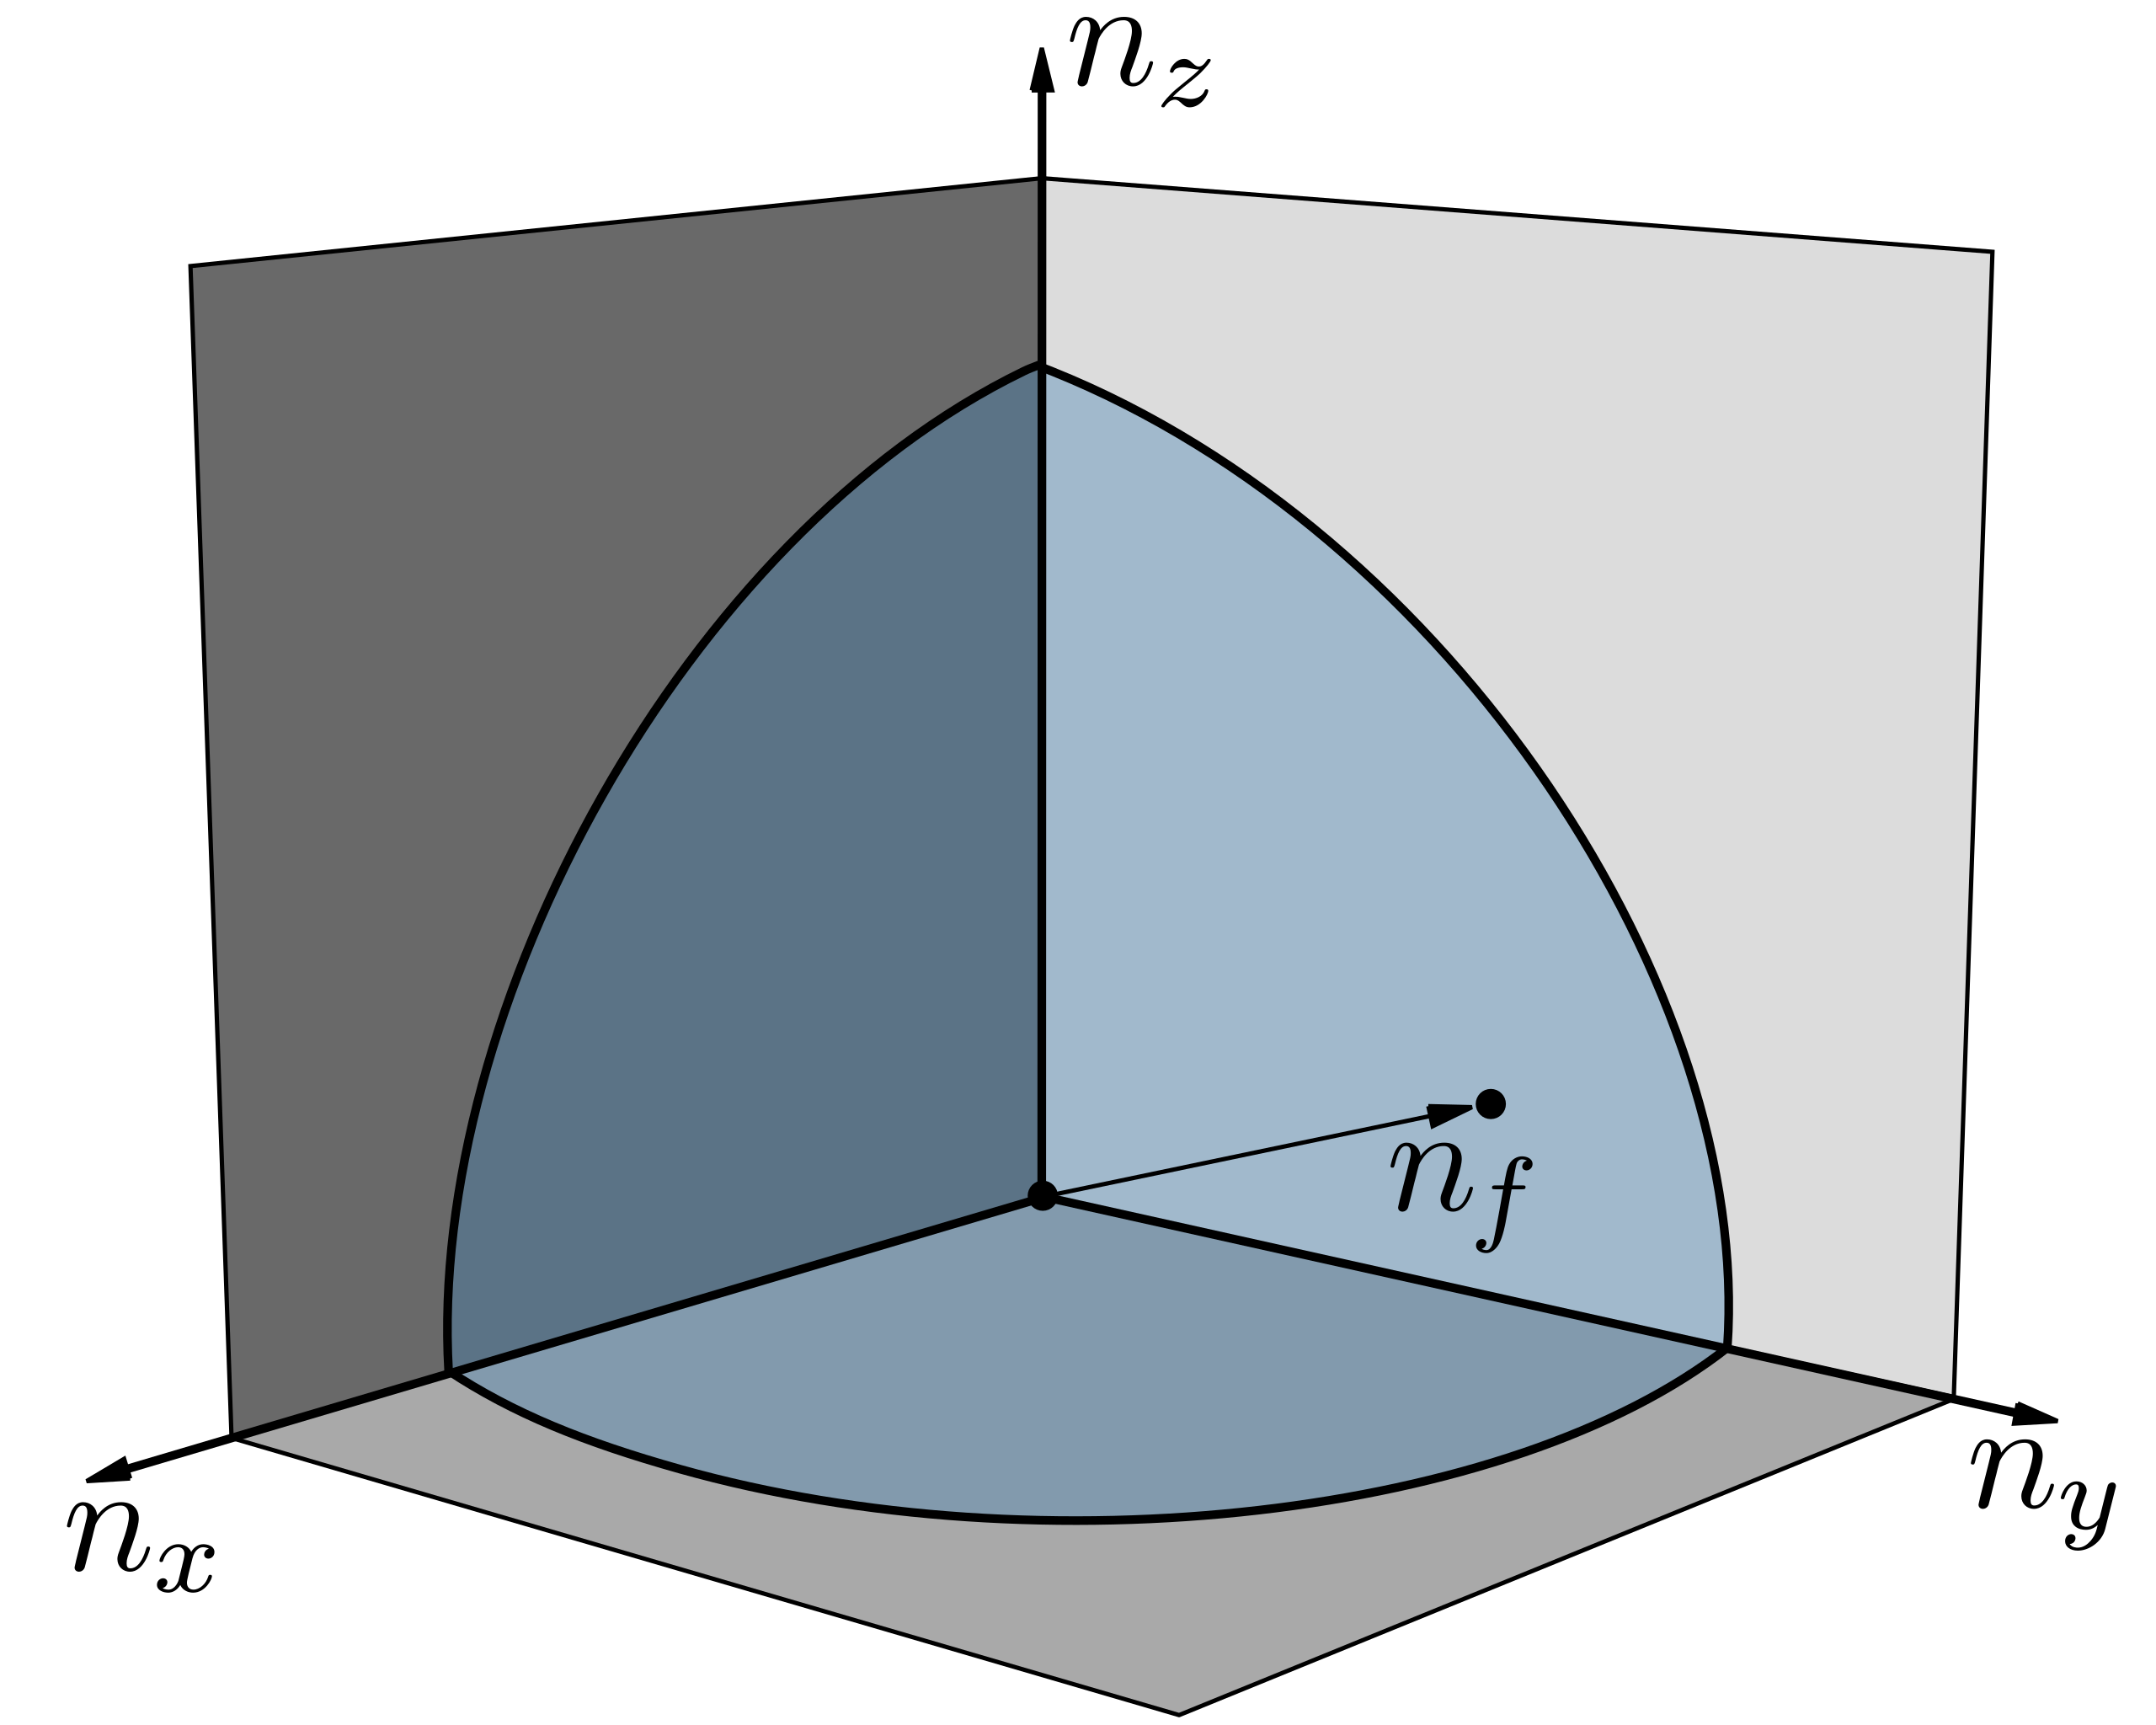
\includegraphics{figs/Fermi-surface}
	    \caption{Fermi surface.}
%	\label{fig:goccia1}
\end{marginfigure}
Dato che, secondo il principio di esclusione di Pauli, ciascuno stato quantistico della funzione d’onda orbitale può alloggiare al massimo due fermioni identici (uno per ciascuno dei due stati di spin del nucleone descritti da uno spinore che abbiamo omesso) concludiamo che \textbf{il numero di neutroni o protoni identici che possono essere contenuti nel volume nucleare V di superficie S con valore massimo dell’impulso} $P_f$ è dato dalla espressione seguente
\begin{equation}
	n_{f} = \frac{V P_{F}^{3}}{3 \pi^{2}\hslash^{3}} \left( 1 - \frac{3\pi \hslash}{4} \frac{S}{VP_{F}} \right)
	\label{eq:fermions-number-specified-volume-momentum}
\end{equation}

Essa costituisce la formula fondamentale del modello a gas di fermioni, base di ogni successivo sviluppo del modello stesso.
La (\ref{eq:fermions-number-specified-volume-momentum}) permette di stimare immediatamente alcune grandezze fisiche fondamentali del modello. Trascurando il termine di superficie che si può mostrare essere assi più piccolo di quello di volume, ricaviamo l’espressione \emph{dell’impulso di fermi in funzione del numero di fermioni nucleari}( tenendo conto del fatto che $\frac{\hslash S}{V} \ll 1$)
\begin{equation}
	P_{F} \simeq \hslash \left(\frac{3\pi^{2}n_{F}}{V} \right)^{1/3}
	\label{eq:fermi-momentum-estimate}
\end{equation}
Le ipotesi di \emph{stabilità} del nuclide e dell'occupazione dello \emph{stato di minima energia} si traducono in
\[
	V \simeq \frac{4}{3}\pi r_{0}^{3}A \quad e \quad n_{p}\simeq n_{s} \simeq \frac{A}{2}
\]
per cui usando la (\ref{eq:fermi-momentum-estimate}) possiamo ottenere una stima del valore \textbf{dell’impulso di Fermi} dei protoni e neutroni nucleari
\[
P_{F} = \left( \frac{9\pi}{8} \right)^{1/3} \frac{\hslash}{r_{0}} \simeq 1.52 \frac{\hslash}{1.2 \times \frac{1}{200}\frac{\hslash c}{MeV}} \simeq 254 \frac{MeV}{c}
\]
Dunque, \emph{nel nucleo prossimo allo stato fondamentale, esiste una frazione di nucleoni con un impulso piuttosto rilevante}. Inoltre, \emph{l’impulso di Fermi dei protoni e neutroni risulta essere indipendentemente dal tipo e dimensioni del nucleo}, un fatto che non ci sorprende solo a posteriori.
\bigskip

E’ immediato allora stimare la \textbf{energia cinetica di Fermi} dei protoni e neutroni nucleari
\begin{equation}
	E_{F} = \frac{P_{F}^{2}}{2M_{n,p}} \simeq 34 \, MeV
	\label{eq:fermi-kinetic-energy-estimate}
\end{equation}
%Nel caso del nuclepiù semplice ($H$) si avrà che
%%%TODO 20/12/22 niccolozanotti: farsi spiegare da marco cosa scrivere qui
ed anche la \textbf{profondità della buca di potenziale nucleare} che sarà approssimativamente uguale alla somma della energia di Fermi con la energia media di separazione dei nucleoni che vale circa $8 \, MeV$
(vedi Fig.~\ref{fig:en-legame-graph})
\begin{equation}
	V_{0} \simeq E_{F} + \frac{B}{A} \simeq (34 + 8)\, MeV \simeq 42 \, MeV
   \label{eq:}
\end{equation}
entrambi indipendenti da A \emph{e dunque approssimativamente valide per tutti i nuclei}.

\subsection{L'espressione dell'energia di legame}\label{subsec:energia-di-legame-fermions-gas}

Si noti che l’energia cinetica dei nucleoni non è molto inferiore alla profondità della buca (è inferiore di 8 MeV appunto) per cui \emph{il nucleo è un insieme di nucleoni debolmente legati}.

Nel caso dei nuclei stabili pesanti dobbiamo tenere conto che il numero di neutroni eccede quello dei protoni per cui dalla (\ref4.30) e (\ref4.31) otteniamo \emph{che l’impulso e la energia di Fermi dei neutroni supera quello dei protoni}
\[
P_{F}^n > P_{F}^p \qquad E_{F}^n > E_{F}^p
\]
e così pure per la (\ref4.32) \emph{la profondità della buca di potenziale dei neutroni supera quella dei protoni}
\[
V_{0}^n > V_{0}^p
\]
Se ora teniamo conto che i protoni - a causa della carica elettrica che possiedono - sono soggetti ad un potenziale repulsivo coulombiano sostanzialmente apprezzabile solo
quando quello nucleare si azzera, abbiamo che i potenziali complessivi di
neutroni e protoni devono avere l’andamento approssimato mostrato in Figura~\ref{fig:fermi-gas-model-potential-scheme}.

\begin{figure}
	\centering
	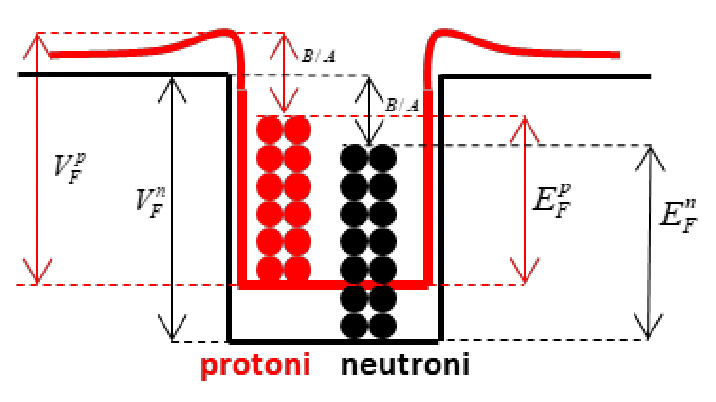
\includegraphics{../figs/fermi-gas-model-potential-scheme}
	\caption{Scheme of Fermi gas model potential.}
	\label{fig:fermi-gas-model-potential-scheme}
\end{figure}

Queste considerazioni chiariscono le linee di ragionamento che possono condurre alla costruzione della \emph{formula della energia di legame basata sul modello a gas di fermioni}.

Un \textbf{neutrone porta un contributo medio alla energia di legame nucleare} pari alla differenza tra la profondità della buca di potenziale e la sua energia cinetica media
\[
b_{n} = V_{0} - \langle T_{n} \rangle
\]
Per un protone si deve ragionare allo stesso modo aggiungendovi però la repulsione coulombiana che rende la buca del potenziale totale meno profonda.
La repulsione coulombiana media per protone ha la seguente espressione (8-1 Feynman\cite{FeynLect2})
\[
	\langle V_{coul} \rangle = \frac{1}{Z} \mathlarger{\sum}_{\substack{j,k=1 \\ j \neq k, \,j > k  }}^{Z} \frac{e^{2}}{4 \pi \epsilon_{0}r_{jk}}\]
e dipende dalla disposizione spaziale dei protoni.
Ipotizzando una distribuzione spazialmente uniforme (problema della sfera uniformemente carica) otteniamo
\[
U_{coul}^{tot} = \frac{3}{5} \frac{e^{2}}{4 \pi \epsilon_{0}} \frac{Z^{2}}{R} = \frac{3}{5} \frac{e^{2}}{4 \pi \epsilon_{0} \hslash c} \hslash c \frac{Z^{2}}{R} = \frac{3}{5} \alpha \hslash c \frac{Z^{2}}{R}
\]
dove $\alpha \simeq \frac{1}{137}$ è la \emph{costante adimensionale di struttura fina} e $R$ è il raggio della distribuzione sferica di carica ovvero il raggio nucleare.
Invocando un ragionamento già fatto per il modello a goccia quando si è parlato del termine coulombiano (si veda (\ref{eq:work-to-seperate-uniformly-distributed-protons})) nel nostro modello la precedente si riscrive come
\[
U_{coul}^{tot} = \frac{3}{5} \alpha \hslash c \frac{Z (Z-1)}{R} \ \cdot
\]
Possiamo ora scrivere il \emph{contributo medio del protone alla energia di legame nucleare} $b_{p}$\sidenote
{
Osserviamo che $ b_n$ e $ b_p$ sono stati stimati teoricamente a partire dal modello a gas di Fermi e non tramite
considerazioni sul difetto di massa come in precedenza. Di fatto si vuole migliorare il precedente modello fenomenologico
(a goccia) cercando di ricavare la dipendenza di $ B$ da $ A$ e $ Z$.
}
\begin{gather*}
    \langle U^{tot}_{coul} \rangle = \frac{U^{tot}_{coul}}{Z}\\
    b_{p} = V_{0} - \langle T_{p} \rangle  - \frac{1}{Z}
\end{gather*}
Tenendo ora conto espressione e dell’analoga per i neutroni possiamo comporre la seguente \textbf{espressione della energia di legame nucleare}
\begin{equation}
	B = N b_{n} + Z b_{p} = A V_{0} - N \langle T_{n} \rangle - Z \langle T_{p} \rangle - \frac{3}{5} \alpha \hslash c \frac{Z(Z-1)}{R}
	\label{eq:binding-energy-fermi-gas-model}
\end{equation}


\subsection{Il calcolo dell'energia di legame}\label{sec:calcolo-energia-legame-fermions-gas}



\section{Il modello a Shell}\label{sec:il-modello-a-shell}


